%%%%%%%%%%%%%%%%%%%%%%%%%%%%%%%%%%%%%%%%%
% University Assignment Title Page 
% LaTeX Template
% Version 1.0 (27/12/12)
%
% This template has been downloaded from:
% http://www.LaTeXTemplates.com
%
% Original author:
% WikiBooks (http://en.wikibooks.org/wiki/LaTeX/Title_Creation)
%
% License:
% CC BY-NC-SA 3.0 (http://creativecommons.org/licenses/by-nc-sa/3.0/)
% 
% Instructions for using this template:
% This title page is capable of being compiled as is. This is not useful for 
% including it in another document. To do this, you have two options: 
%
% 1) Copy/paste everything between \begin{document} and \end{document} 
% starting at \begin{titlepage} and paste this into another LaTeX file where you 
% want your title page.
% OR
% 2) Remove everything outside the \begin{titlepage} and \end{titlepage} and 
% move this file to the same directory as the LaTeX file you wish to add it to. 
% Then add \input{./title_page_1.tex} to your LaTeX file where you want your
% title page.
%
%%%%%%%%%%%%%%%%%%%%%%%%%%%%%%%%%%%%%%%%%
%\title{Title page with logo}
%----------------------------------------------------------------------------------------
%	PACKAGES AND OTHER DOCUMENT CONFIGURATIONS
%----------------------------------------------------------------------------------------

\documentclass[12pt]{article}
\usepackage[english]{babel}
\usepackage[utf8x]{inputenc}
\usepackage{amsmath}
\usepackage{graphicx}
\usepackage{movie15}
\usepackage{datetime}
\usepackage{hyperref}
\usepackage[colorinlistoftodos]{todonotes}

\begin{document}

\begin{titlepage}

\newcommand{\HRule}{\rule{\linewidth}{0.5mm}} % Defines a new command for the horizontal lines, change thickness here

\center % Center everything on the page
 
%----------------------------------------------------------------------------------------
%	HEADING SECTIONS
%----------------------------------------------------------------------------------------


\includegraphics[width=0.6\textwidth]{ecn.png}

%----------------------------------------------------------------------------------------
%	TITLE SECTION
%----------------------------------------------------------------------------------------

\HRule \\[0.4cm]
{ \huge \bfseries OPTEC Labs : Optimization of a trajectory AB inside a 10x10 room by avoiding collisions against obstacles using MATLAB}\\[0.4cm] % Title of your document
\HRule \\[1.5cm]
 
%----------------------------------------------------------------------------------------
%	AUTHOR SECTION
%----------------------------------------------------------------------------------------

\begin{minipage}{0.4\textwidth}
\begin{flushleft} \large
\emph{Author:}\\
Thomas \textsc{MARQUET} % Your name
Leonid \textsc{LIANOU}
\end{flushleft}
\end{minipage}
~
\begin{minipage}{0.4\textwidth}
\begin{flushright} \large
\emph{Supervisor:} \\
Fouad \textsc{Bennis} % Supervisor's Name
\end{flushright}
\end{minipage}\\[2cm]

% If you don't want a supervisor, uncomment the two lines below and remove the section above
%\Large \emph{Author:}\\
%John \textsc{Smith}\\[3cm] % Your name

%----------------------------------------------------------------------------------------
%	DATE SECTION
%----------------------------------------------------------------------------------------
\newdate{date}{20}{05}{2019}
{\large \displaydate{date}}\\[2cm] % Date, change the \today to a set date if you want to be precise

%----------------------------------------------------------------------------------------
%	LOGO SECTION
%----------------------------------------------------------------------------------------

% Include a department/university logo - this will require the graphicx package
 
%----------------------------------------------------------------------------------------

\vfill % Fill the rest of the page with whitespace

\end{titlepage}



\begin{figure}
\vspace{-10mm}
\section{Introduction}

The purpose of this lab is to understand how to use the function fmincon and the methodology around it. But also to know the limits of this tool.
\vspace{5mm}

To implement the obstacles we choosed to use fixed starting point, end point and circles because it is more consistent. The optimized path is in red and the guessed trajectory is in green.
\vspace{5mm}
Comments about the code on himself are in the code.(discretization inside contraint4, fmincon and its arguments inside project-main-final, and objective function in obj4).
\vspace{5mm}
\section{First step : 1 circle and 1 guess point}
As you can see below it is really simple :

\begin{center}
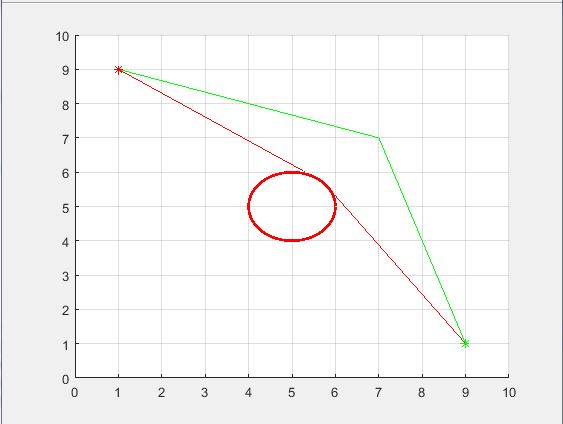
\includegraphics[width=1\textwidth]{level1.JPG}
\end{center}
\vspace{5mm}
We observed that the optimized path could be either going over the circle or under the circle. It is a simple phenomenon of local minimum depending on the guess points. If the guess points are mostly over the circle, then the final path would be over the circle even if going down would be even more optimized.

\end{figure}

\begin{figure}
\vspace{-10mm}

\section{Second step : 2 circles and 5 guess points}
For this step, we've got five guess points so because of the weird shape of the initial trajectory and the randomness of the guess points, it gets less consistent. points.

\begin{center}
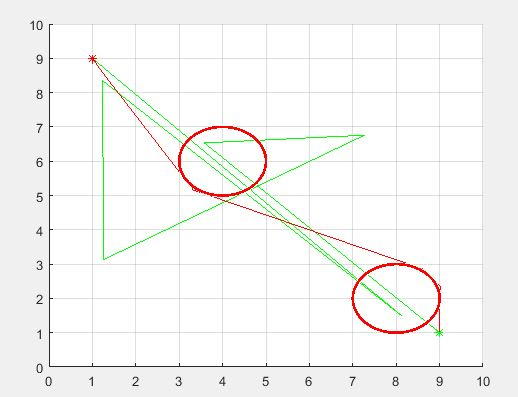
\includegraphics[width=1\textwidth]{level2.JPG}
\end{center}

Same as before, the optimized path highly depends on where are the initials points but in this case convergence of the path is not systematic also because of the guess points.
\vspace{5mm}




\end{figure}


\begin{figure}
\vspace{-10mm}

\section{Third step : 4 circles and 7 guess points}
Just like the second step, the more we add obstacles and randomness into the problem, the less it is consistent.

\begin{center}
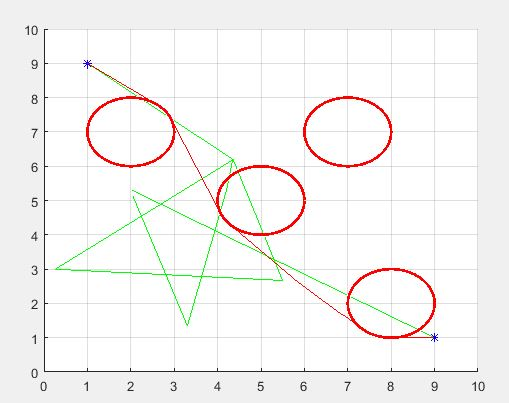
\includegraphics[width=1\textwidth]{level3.JPG}
\end{center}

Same as before, the optimized path highly depends on where are the initials points.
\vspace{5mm}
\section{Final step : 4 circles and walls}
For the final step, the methodology is quite different since we now have walls and it is adding a lot more difficulties to converge. So we've to help the algorithm by fixing the right boundaries to the initials guess points. We can have, for example, on  7 guess points : 2 guess points on the left of the walls, 2 on the right, 1 at the entry of the corridor, 1 in the middle of the corridor and 1 at the end.
\end{figure}
\begin{figure}
\vspace{-10mm}

 The "head start" we're giving to the algorithm is a critical condition on its convergence.

\begin{center}
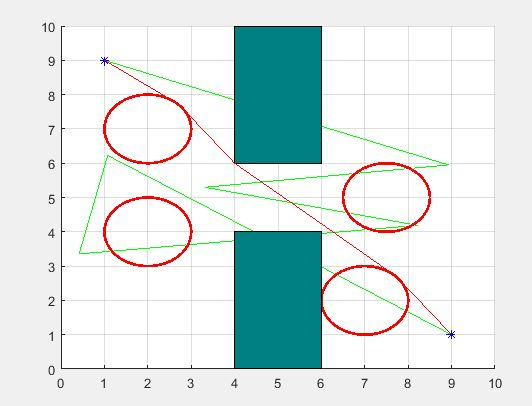
\includegraphics[width=1\textwidth]{final.JPG}
\end{center}

Same as before, the optimized path highly depends on where are the initials points. But since here the guess points are less "free", the path is most likely to be similar on each try.
\vspace{5mm}
\section{Conclusion :}
We can see that in every case the path depends on the guess points. With two differents sets of guess points we can have drastically differents solutions and even solutions that would never have been taken by an human (really far from global minimum). I guess a good solution to improve this would be to take multiple convergent paths and compare them to get the best answer between all of them. Or you could also get your initial guess point using known acceptable guess points(like in the final solution).


\end{figure}
\end{document}